\section{Exact broad search space}
\label{app:search}

\begin{figure*}[t]
  \centering
  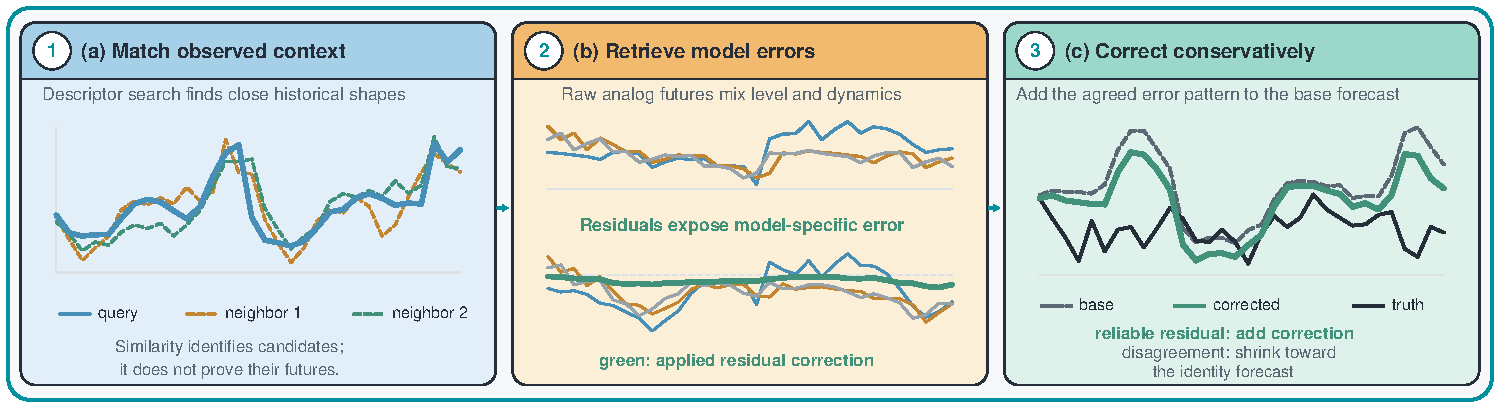
\includegraphics[width=\textwidth]{figures/residual_retrieval_example.pdf}
  \caption{\textbf{Residuals isolate model-specific error on real data.} An
  ETTh1 MULL example from a frozen TimeMixer. (a) Descriptor search returns
  historical windows with closely matching shapes. (b) Their raw futures sit at
  different levels and mix dynamics the base forecast already captures, whereas
  their residuals agree on a common error pattern. (c) Adding the shrunk
  residual moves the forecast toward the truth without disturbing its level.
  Panels (b)--(c) show a 36-step excerpt in the model's standardized space.}
  \label{fig:residual-example}
\end{figure*}

\begin{figure*}[t]
\hrule\vspace{2pt}
\textbf{Algorithm 1:} \method{} calibration and forecast-time revision\\[1pt]
\hrule\vspace{3pt}
\textbf{Input:} frozen forecaster $f$; validation stream
$\{(\xctx_i,\ytrue_i)\}$; candidate families and grids; metric set
$\mathcal{Q}$.\\
\textbf{Calibration.}
(1) For every validation origin $i$, evaluate $\ybase_i=f(\xctx_i)$ and, once
$\ytrue_i$ has fully elapsed, store
$(\feat_i,\ybase_i,\resid_i=\ytrue_i-\ybase_i)$ in $\mathcal{M}$.
(2) Split $\mathcal{M}$ chronologically into a memory prefix and a query
suffix.
(3) For each candidate $c$, form $\ycorr^{(c)}$ on the query suffix using only
the memory prefix and score it by $S(c)$.
(4) Lock the minimizing family and parameters $c^\star$; ties go to identity.\\
\textbf{Forecasting at origin $t$.}
(5) Evaluate $\ybase_t=f(\xctx_t)$ and build $\feat_t$ from $\xctx_t$ and
$\ybase_t$.
(6) If $c^\star$ is retrieval, take the top-$k$ items of $\mathcal{M}_t$ with
$i+H<t$, aggregate by Equation~\ref{eq:weights} and shrink by
Equation~\ref{eq:shrinkage}; otherwise evaluate the locked simpler correction.
(7) Return $\ycorr_t=\ybase_t+c_t$, leaving $f$ unchanged.\\
\vspace{1pt}\hrule
\end{figure*}

The ETTh1 example in Figure~\ref{fig:residual-example} was screened
deterministically for visualization only; the screening criteria and score
weights are recorded in the released case artifact and never enter method
selection.

\begin{table*}[h]
\centering
\small
\caption{Validation-only candidate space for the broad selector.}
\label{tab:search-space}
\begin{tabular}{p{0.22\textwidth}p{0.65\textwidth}}
\toprule
Family & Candidate values\\
\midrule
Identity & No parameters\\
Residual descriptor & Tail $\ell\in\{\min(48,L),L\}$; pooled steps
$\min(12,\ell)$; differences on; base forecast on/off; calendar on except PEMS;
at most 16 pooled channels\\
Residual aggregation &
$(k,\tau,\lambda)\in\{(8,0.1,1),(16,0.3,4)\}$;
$\alpha\in\{.05,.1,.2,.3,.5\}$\\
Seasonal blend & Long-term periods $\{4,8,12,24,48,96,168\}$, PEMS periods
$\{12,24,48,96\}$, and EPF periods $\{24,48,168\}$, each clipped at $L$ and
deduplicated; $\alpha\in\{.02,.05,.1,.2,.3\}$\\
Overlap blend & $(a,\gamma)\in\{(8,.75),(24,.9)\}$;
$\alpha\in\{.1,.25,.5\}$\\
Static residual bias & $\alpha\in\{.1,.25,.5,1\}$\\
Causal rolling bias & Window $W\in\{2H,8H,32H\}$; horizon block
$b\in\{0,\min(24,H)\}$; $\alpha\in\{.1,.25,.5,1\}$\\
\bottomrule
\end{tabular}
\end{table*}

\begin{table*}[h]
\centering
\small
\setlength{\tabcolsep}{5pt}
\caption{Information available to each correction candidate at forecast
origin $t$. A label is eligible only after its target timestamp has passed.}
\label{tab:candidate-availability}
\begin{tabular}{p{0.22\textwidth}p{0.68\textwidth}}
\toprule
Candidate & Information used\\
\midrule
Identity & Current frozen-model prediction only; no labels\\
Seasonal blend & Observed context through $t$; no labels\\
Overlap blend & Predictions issued at earlier origins for the same target
timestamps; no labels\\
Static residual bias & Validation predictions and validation labels\\
Historical residual retrieval & Validation contexts, predictions, and labels\\
Causal rolling bias & Validation evidence and test labels with target time
$u<t$\\
ETTm post-test retrieval & Validation evidence and completed official-test
residuals; no post-test label with target time $u\ge t$\\
ETTh online stack & Training data for NLinear, earlier predictions of the same
targets, and delayed labels with target time $u<t$\\
\bottomrule
\end{tabular}
\end{table*}

\paragraph{Temporal-candidate parameters.}
For overlap blend, $a$ is the maximum age in forecast origins and $\gamma$ is
the per-origin exponential decay. For causal rolling bias, $W$ is the
target-time lookback. Setting $b=0$ pools all forecast leads; otherwise,
contiguous groups of $b$ leads receive separate bias estimates. The grouping
changes which completed errors are averaged, not when a label becomes
eligible.

\paragraph{Chronological validation partition.}
Let validation contain $n$ forecast windows. The query suffix begins at
$\max(\lfloor n/2\rfloor,H+8)$, adjusted to stay below $n$. The residual
memory ends at least $H$ origins earlier, so every memory future is complete.
The final test retriever is fit on the complete validation split because that
split precedes test.

\paragraph{Selection tie breaking.}
Candidates minimize the worst-metric validation ratio $S(c)$ of
Section~\ref{sec:selection}. Identity wins an exact
score tie. When the best score is at least 0.982, only candidates improving
all validation metrics are eligible for family-prior selection. Within a
family, the lowest score wins; the family order is overlap, seasonal,
historical residual, static residual bias, and causal rolling bias.

\paragraph{Internal policy holdout.}
The supplementary material lists the fixed 123 development and 462 holdout
cell IDs. Membership uses the first 123 completed cells ordered by
\texttt{started\_unix} and does not use any metric value. The boundary is
nevertheless an opportunistic execution-order split rather than a stratified
dataset, model, or difficulty holdout. Its scope and balance diagnostics are
reported in Appendix~\ref{app:aggregate-results}.
